
要构建项目,应该从清楚地了解将在其中创建什么逻辑目标开始。本例中,将遵循图12.2所示的结构:

\begin{center}
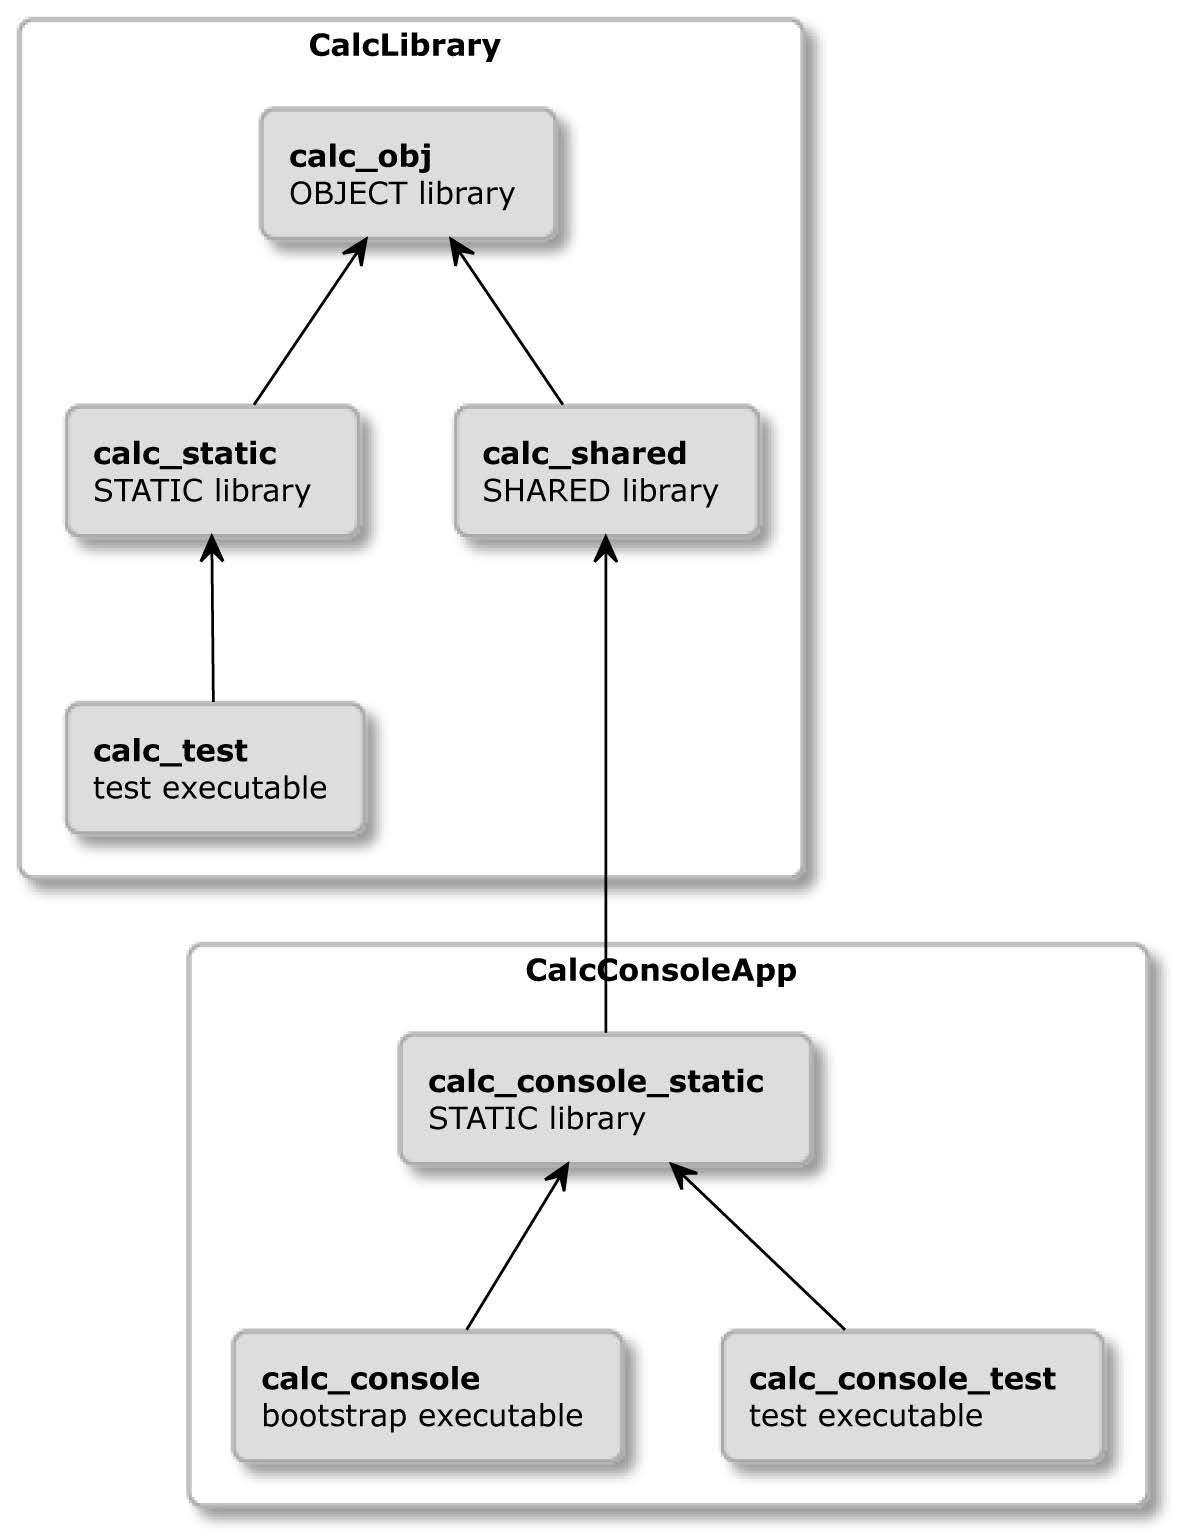
\includegraphics[width=0.6\textwidth]{content/3/chapter12/images/2.jpg}\\
图12.2 逻辑目标的结构
\end{center}

我们按照构建顺序来探索这个结构。首先,编译calc\_obj,这是一个对象库。我们确实在书中几次提到了对象库,但并没有作为一个知识点来介绍。

\subsubsubsection{12.3.1\hspace{0.2cm}对象库}

对象库用于将多个源文件分组到单个逻辑目标下,并在构建期间编译到(.o)目标文件中。要创建一个对象库,使用OBJECT关键字与其他关键字相同:

\begin{lstlisting}[style=styleCMake]
add_library(<target> OBJECT <sources>)
\end{lstlisting}

构建过程中产生的对象文件可以通过\$<TARGET\_OBJECTS:objlib>生成器表达式作为编译后的元素添加到其他目标:

\begin{lstlisting}[style=styleCMake]
add_library(... $<TARGET_OBJECTS:objlib> ...)
add_executable(... $<TARGET_OBJECTS:objlib> ...)
\end{lstlisting}

或者,可以使用target\_link\_libraries()将其作为依赖项添加。

Calc库中,对象库将有助于避免为库的静态和动态版本重复编译库源。只需要记住显式地使用POSITION\_INDEPENDENT\_CODE编译目标文件,因为这是动态库的需求。

解决了这些问题,回到这个项目的目标:calc\_obj将提供编译的目标文件,然后将用于calc\_static和calc\_shared库。它们之间的实际区别是什么?为什么要提供两个库?

\subsubsubsection{12.3.2\hspace{0.2cm}比较动态库与静态库}

第6章中简要介绍了这两种类型的库,对于使用相同动态库的多个程序,整体内存使用可能会更好,而且用户很可能已经拥有最流行的库,或者知道如何快速安装。更重要的是,动态库是在单独的文件中交付的,这些文件必须安装在特定的路径中,以便动态链接器找到,而静态库是作为可执行文件的一部分,因为不需要在内存中查找代码的位置,所以静态库使用起来稍微快一些。

作为库作者,可以决定是提供库的静态还是动态版本,或者可以简单地提供两个版本,并把这个决定留给使用库的开发者。我们在这里选择后者(只是为了了解如何完成)。

静态库将由calc\_test目标使用,该目标将包含单元测试,以确保所提供的库业务功能按预期工作。我们从同一组已编译的目标文件构建两个版本,测试任何一个都可以,因为其行为没有区别。

由calc\_console\_static目标提供的控制台应用程序将使用动态库。该目标还将链接到一个外部依赖:Arthur Sonzogni的功能终端用户界面(FTXUI)库(在扩展阅读部分有一个到GitHub项目的链接)。它为文本用户界面提供了一个无依赖性、跨平台的框架。

最后两个目标是calc\_console和calc\_console\_test。calc\_console目标只是一个围绕calc\_console\_static的bootstrap main()包装器,其目的是从业务代码中提取入口点。可以为其编写单元测试(需要提供接口),并使用calc\_console\_test运行。

现在知道需要建立什么目标,以及它们之间的关系。来看看如何用文件和目录来组织项目。

\subsubsubsection{12.3.3\hspace{0.2cm}目录结构}

该项目包含两个主要目标,calc库和calc\_console可执行文件,每个目标都位于src和test下的目录树中,以将生产代码与测试代码分离(如图12.3所示)。此外,文件放在另外两个目录中:

\begin{itemize}
\item 
包含顶层配置和关键项目文档文件的根目录

\item 
cmake目录中包含用来构建和安装项目的所有工具模块和帮助文件:

\begin{center}
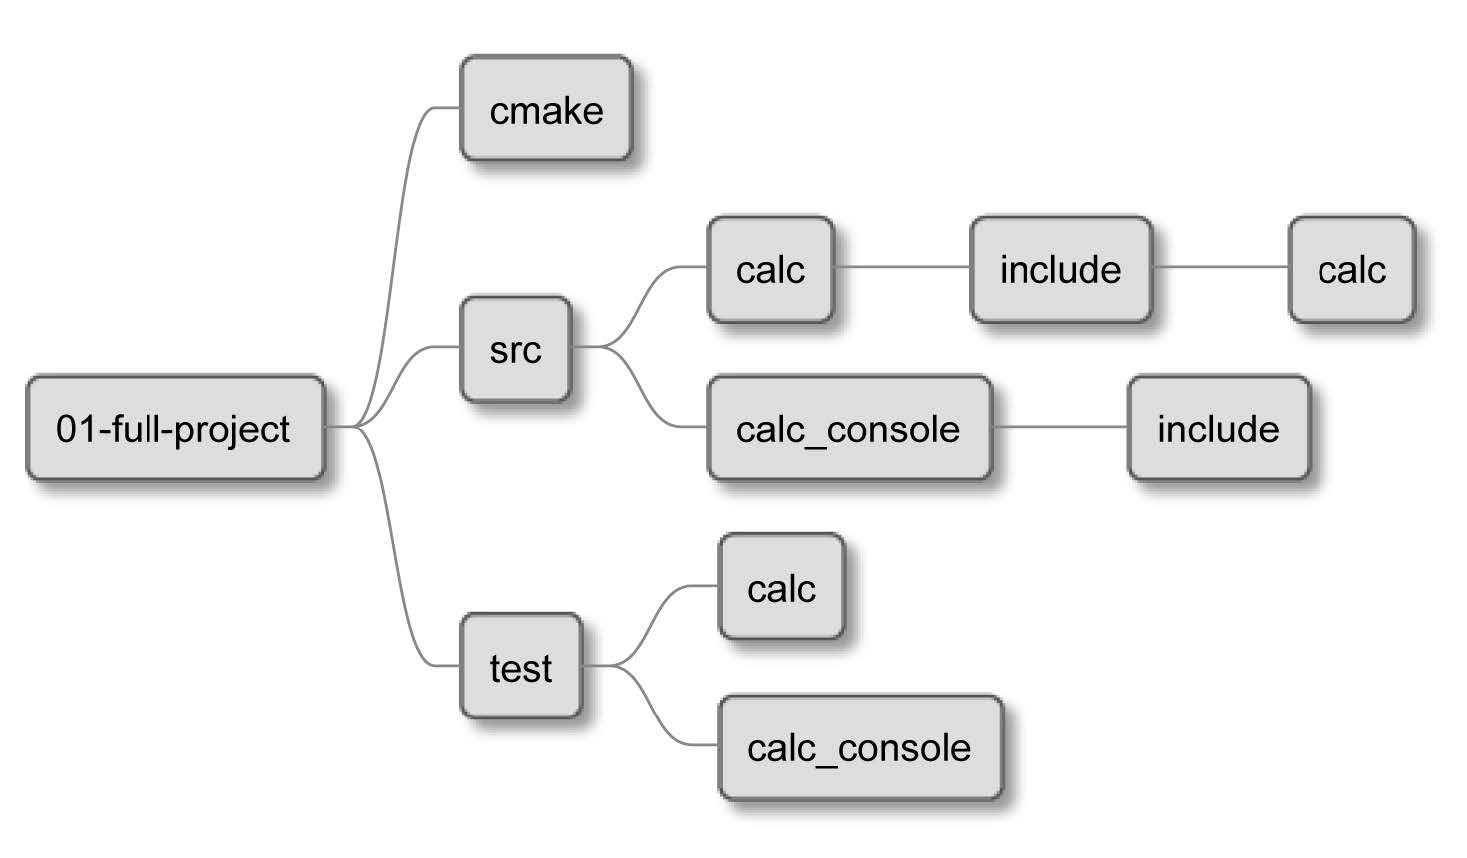
\includegraphics[width=0.6\textwidth]{content/3/chapter12/images/3.jpg}\\
图12.3 项目的目录结构
\end{center}
\end{itemize}

以下是四个主目录下文件的完整列表:

\begin{table}[H]
	\centering
	\begin{tabular}{|l|l|}
		\hline
		\textbf{./}    & \textbf{./test}  \\ \hline
		\begin{tabular}[c]{@{}l@{}}CHANGELOG\\ CMakeLists.txt\\ CalcConfig.cmake\\ INSTALL\\ LICENSE\\ README.md\end{tabular} &
		\begin{tabular}[c]{@{}l@{}}CMakeLists.txt\\ calc/CMakeLists.txt\\ calc/calc\_test.cpp\\ calc\_console/CMakeLists.txt\\ calc\_console/tui\_test.cpp\end{tabular} \\ \hline
		\textbf{./src} & \textbf{./cmake} \\ \hline
		\begin{tabular}[c]{@{}l@{}}CMakeLists.txt\\ calc/CMakeLists.txt\\ calc/calc.cpp\\ calc/include/calc/calc.h\\ calc\_console/CMakeLists.txt\\ calc\_console/bootstrap.cpp\\ calc\_console/include/tui.h\\ calc\_console/tui.cpp\end{tabular} &
		\begin{tabular}[c]{@{}l@{}}buildinfo.h.in\\ BuildInfo.cmake\\ Coverage.cmake\\ CppCheck.cmkae\\ Doxygen.cmake\\ Format.cmake\\ GetFTXUI.cmake\\ Install.cmake\\ Memcheck.cmake\\ NoInSourceBuilds.cmake\\ Testing.cmake\end{tabular} \\ \hline
	\end{tabular}
\end{table}

最初,cmake目录比业务代码更多,但随着项目功能的增长,这种情况将很快发生变化。启动一个清洁项目的努力是很重要的,但不要担心——很快就会得到回报。

我们将浏览所有文件,详细了解它们的作用以及它们在项目中扮演的角色。这将分为四个步骤:构建、测试、安装和生成文档。















